%%================================================
%% Filename: chap03.tex
%% Encoding: UTF-8
%% Author: Yuan Xiaoshuai - yxshuai@gmail.com
%% Created: 2012-04-27 19:47
%% Last modified: 2019-11-07 14:38
%%================================================
\chapter{基于接口号分组的概率标记法}
\label{cha:IGPPM}


传统的PPM(概率包标记法)通常使用路由器的IP地址作为标记信息,然而IP地
址是相对于全球的网络设备的,占用空间大,为32 bit。故PPM通常只会携带一
个路由器的标记信息,这导致了概率包标记法的空间利用率较低,为$1/32 = 
0.03125$。这也是为什么传统的概率包标记法需要收集更多数据包以进行路径
重构的原因。

在本文中,我们将采用一种不同的方法:利用路由器的接口号作为标记信息。IP
地址是相对于全球网络设备的,而路由器接口号仅相对于单个路由器内的所有网
络接口,所以对单个路由器内的每个接口进行编码将消耗更少的空间。这意味着
我们可以在一个数据包中标记多个路由器的信息,提高了标记空间的利用率,从
而提高了路径重构的效率,减少了需要收集的数据包数量。这将显著改善数据包
标记法进行IP回溯的性能和有效性。

\section{标记字段数据结构}

图~\ref{fig:data_structure}~展示了本方案标记空间所采用的抽象数据结构。标记空间具体来自于数据包头部字段,在实际应用时可以依照图2中的IP头部字段来构建此标记空间。在本方案中,我们利用数据包头部中的 b bit来标记数据包经过的路由器来源接口号。每个数据包携带了 m 个接口号标记字段以及两个 XOR (异或)字段,每个 XOR 字段也占据 b bit。最后,还有一个 1 位的允许标志位。总的标记空间大小为 $l = 1 + (m + 2) \times b$ bit,用于支持数据包标记过程。
\begin{figure}[htbp]
  \centering
  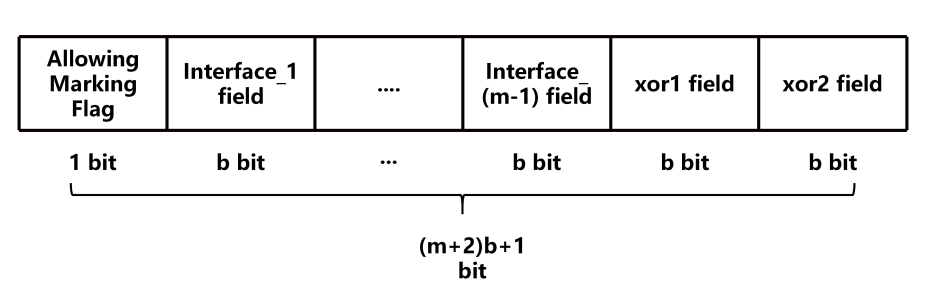
\includegraphics[width = 0.8\textwidth]{data_structure}
  \caption{方案所采用的数据结构}
  \label{fig:data_structure}
\end{figure} 

具体的数值 b 和 m 可以根据实际应用场景来确定。在本文的运行示例中,我
们选择了 b = 6,这是因为大多数互联网路由器的接口数量远远少于 $2^6 =
64$个。同时,我们选择了 m 分别为 2 和 4,总共使用了 IP 头部中的 25
和 37 bit。这导致了标记空间的利用率分别为 0.08 和 0.0108。相较于
使用 IP 地址进行标记的标记空间,利用率提高了约 2.56 和 3.46 倍。
% 插入外部代码
% \lstinputlisting[firstline=8,style=lstStyleLaTeX]{main.tex}

\section{路由器标记阶段算法}

在本文的数据包标记法部分,算法~\ref{alg:packet_marking}~提供了详细
的内容,用于中间路由器对数据包进行标记,同时,图
~\ref*{fig:marking_procedure}~抽象地描述了这一过程。这一过程包括以
下关键步骤:

\begin{algorithm}
    \small
    \caption{Packet Marking Algorithm}
        \begin{algorithmic}[1] %每行显示行号
            
            \Require m

            \Require  packet
            % \Comment{待转发的数据包}

            \Require srcInterface
            % \Comment{数据包在路由器中的来源接口号}

            %if
            \If {packet.TTL == 0}   \State 
                Drop the packet and exit this program
            \Else   
                \State  set INITIAL\_TTL the minimum value greater than Packet.TTL from \{32, 64, 128, 255\}
                \State  index = (INITIAL\_TTL - packet.TTL) \% group\_size
                \If  {index == 0} 
                    \If {packet.TTL == INITIAL\_TTL} \State
                        set all interface  mark fields to empty \State
                        packet.interfaces[0] = srInterface \State
                        packet.xor1 = srInterface \State
                        packet.allowing\_marking = True
                    \ElsIf{packet.allowing\_marking == True}   \State
                        r = random.random()
                        \If{r $<$ marking\_rate} \State
                            set all interface  mark fields to empty \State
                            packet.interfaces[0] = srInterface \State
                            packet.xor1 = packet.xor1 $\oplus$ srInterface \State
                            packet.allowing\_marking = True
                        \Else \State 
                            packet.allowing\_marking = False
                        \EndIf
                    \EndIf
                \ElsIf{packet.interfaces[index] is empty} \State
                    packet.interfaces[index] = srInterface \State
                    packet.xor1 = packet.xor1 $\oplus$ srInterface
                \EndIf  \State
                packet.TTL -= 1 \State
                packet.xor2 = packet.xor2 $\oplus$ srInterface
            \EndIf
            \State
        \end{algorithmic}
        \label{alg:packet_marking}
    \end{algorithm}

\begin{enumerate}[label=(\alph*).]
  \item \emph{计算路由器位序:}首先,算法需要确定当前路由器是数据包
  所经过路径中的第几个路由器,即当前路由器在数据包需要经过的所有路由
  器的位序。数据包的TTL字段的初始值通常因发送方的系统而异,但通常位于
  范围{32,64,128,255}内。为实现这一步骤,算法首先读取数据包中的
  TTL字段,然后从这组初始值中找到能够不小于数据包TTL的值。然后,计算
  这个最小初始值与数据包中的TTL字段之间的差值,这个差值表示了数据包从
  发送者发送后到达当前路由器时所经过的路由器跳数,即当前路由器在整个
  路径中的位序。
  \item \emph{计算组中序号:}接下来,算法将使用此位序和预定义的组大
  小参数 m(在伪代码中为\emph{group\_size}变量)进行取模运算,得到
  模数。本方案利用路由器在数据包从发送者到受害者的整条路径上的顺序,
  对路由器进行分组。因此,所得的模数表示路由器在组中的序号,范围从0到
  m-1。
  \item \emph{区分路由器类型:}根据功能性需求,路由器可以分为两类:
  组中的0号路由器和非0号路由器。
  \begin{enumerate}
    \item[i.] 对于组中的0号路由器,还需要确定是否是路径中首个路由器。
    如果是首个路由器,便以1概率执行标记操作:将数据包的接口标记字段
    \emph{interface\_0}到\emph{interface\_(m-1)}全部设置为空,即
    未标记状态;将数据包在此路由器中的来源接口号写入到相应的接口标记字
    段;取出XOR1字段中的值与来源接口号进行异或操作,并将结果重新写入到
    XOR1字段;将数据包中的允许标记字段设置为True。如果路由器非首组的0
    号路由器,那么它会根据允许标记字段来决定是否以p概率执行标记操作。若
    标记,操作与前述标记操作相同;若不标记,该路由器会将允许标记字段设置
    为False。这确保了数据包只有经过本组路由器标记后,后面的其它组才有可
    能进行标记。
    \item[ii.] 对于组中非0号路由器,只要数据包中对应的标记字段为空,
    便会对其进行标记:将来源接口号写入到数据包相应的接口标记字段;取
    出XOR1字段中的值与来源接口号进行异或操作,并将结果写入到XOR1字段。
  \end{enumerate}
  \item \emph{更新数据包信息:}最后的步骤适用于所有中间路由器,无论
  是否为组中的0号路由器。具体为将来源接口号与XOR2字段值进行异或运算,
  并将结果重新写入到XOR2字段。这样,XOR2字段结合TTL字段便可作为每条
  路径的地址。在路径重构过程中,以此即可实现对数据包按路径进行分类。
\end{enumerate}

\begin{figure}[htbp]
  \centering
  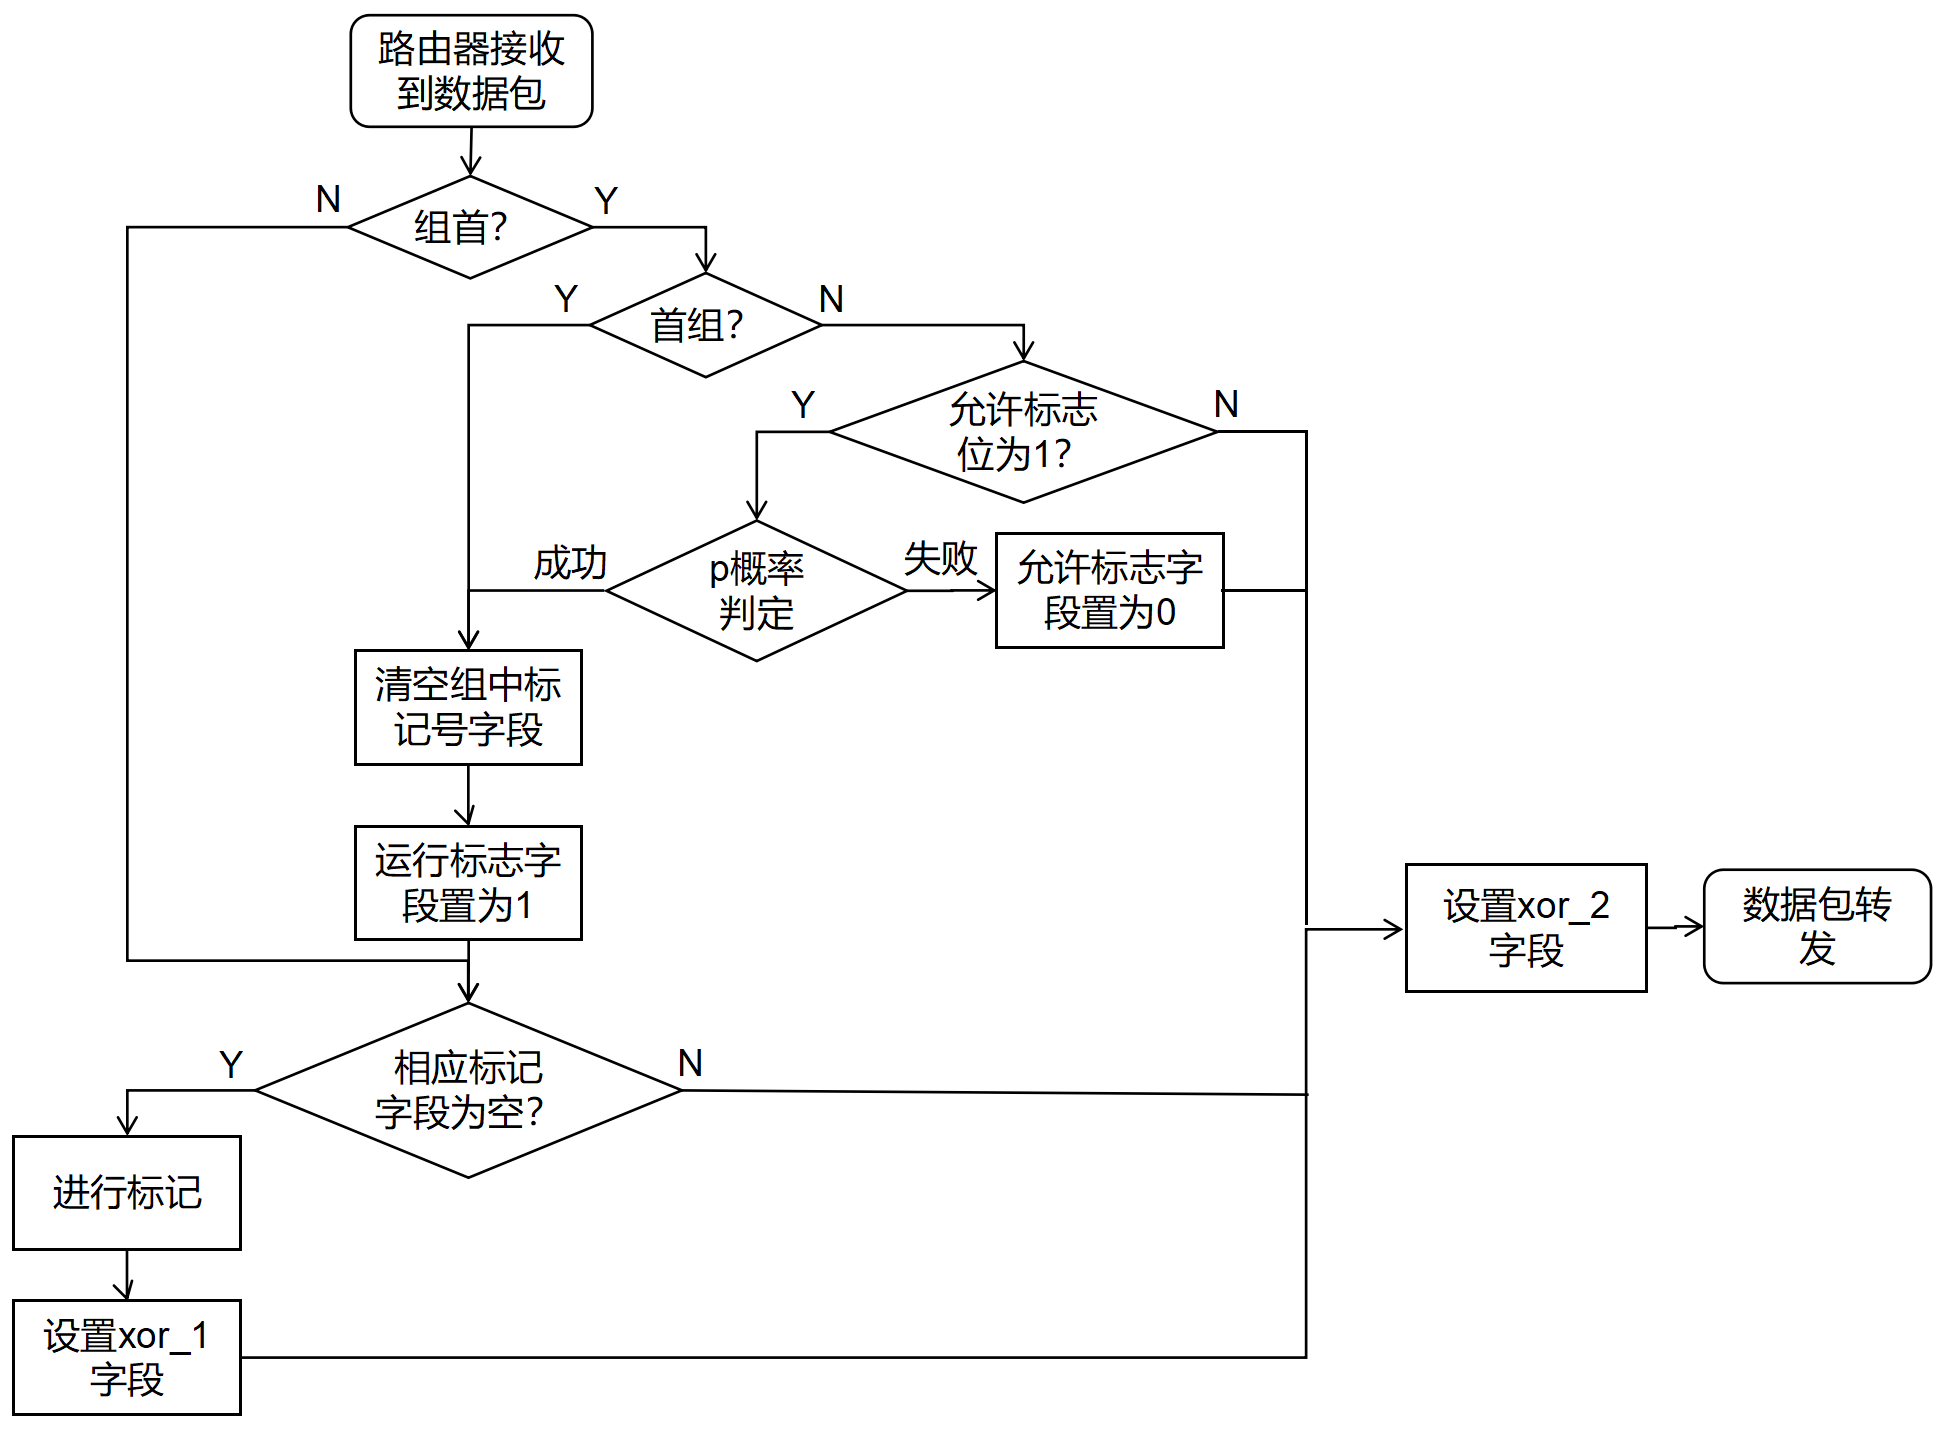
\includegraphics[width = 0.8\textwidth]{marking_procedure.png}
  \caption{算法~\ref{alg:packet_marking}~流程图}
  \label{fig:marking_procedure}
\end{figure}   

\section{路径重组阶段算法}
一旦受害者服务器在检测到攻击后,便会开始收集攻击数据包。当收集到的数
据包数量达到一定阈值时,受害者服务器就会进入收敛状态。在这个状态下,服
务器会利用其中带有标记的攻击数据包来进行路径重构。算法
~\ref{alg:path_reconstruction}~提供了受害者服务器如何在这个过程中
利用标记数据包进行路径重构的详细内容。路径重构的流程为:

\begin{algorithm}[htbp]
    \small
    \caption{Path Reconstruction Algorithm}
    \begin{algorithmic}[1] %每行显示行号

        \Require $S$ \Comment{all marked packets set recived in victim}
        \Ensure $result\_router\_paths$
        \State Initial an empty set $S'$
        \State Initial an empty set $result\_interface\_paths$
        \State Initial an empty set $result\_router\_paths$
        \State is\_multiple\_of\_group\_size = (INITIAL\_TTL - key\_TTL)\%group\_size == 0
        \Comment{Indicate whether the path length is a multiple of the group length}
        \State partition $S$ into different subsets and add in set $S'$ based on packet.TTL and packet.xor2 fields 
        %if
        \For{each subset $U$ in set $S'$} 
            \State Initial an empty set $T$ \Comment{The root data packets used for reconstruction}
            \State  set INITIAL\_TTL the minimum value greater than Packet.TTL from \{32, 64, 128, 255\}
            \For{each packet in subset $U$}
                \State set interface\_count to count of valid interfaces in packet's mark field
                \If{is\_multiple\_of\_group\_size }
                    \If{interface\_count $\not=$ group\_size}
                        \State $U$ = $U$-\{packet\}
                    \ElsIf {packet.xor1==packet.xor2}
                        \State  $T$ = $T$+\{packet\}
                    \EndIf
                \ElsIf {interface\_count $\not=$ group\_size}
                    \State $U$ = $U$-\{packet\}
                    \If {interface\_count == (INITIAL\_TTL - key\_TTL) \% group\_size and packet.xor1 == packet.xor2}
                        \State $T$ = $T$+\{packet\}
                    \EndIf
                \EndIf
            \EndFor
        
            \For {each packet in set $T$}
                \State Initial an empty set $current\_interface\_path$
                \State remaining\_ipath\_length = INITIAL\_TTL - key\_TTL
                \State flag = \Call{try\_construct}{packet, $U$,$result\_interface\_paths$, $current\_interface\_path$,remaining\_ipath\_length}   
                \If{flag == False and is\_multiple\_of\_group\_size}
                    \State $U$ = $U$+\{packet\} \Comment{Restore $U$ to its state before calling 'try\_construct'}
                \EndIf
            \EndFor
        \EndFor
        

        \For{each $interface\_path$ in $result\_interface\_paths$}
            \State current\_router = victim\_router
            \State $reconstructed\_path$ = \{current\_router\}
            \For{each interface\_num in $interface\_path$}
                \If {interface\_num - 1 $<$ len(neighbors,current\_router)}
                    \State next\_router = get\_router\_by\_interface(interface\_num,current\_router)
                    \State $reconstructed\_path$ = $reconstructed\_path$ + \{next\_router\}
                    \State current\_router = next\_router
                \Else
                    \State $reconstructed\_path$ = \{\}
                    \State break
                \EndIf
            \EndFor

            \If {len($reconstructed\_path$) $>$ 0}
                \State $result\_router\_paths$ = $result\_router\_paths$+ reverse($reconstructed\_path$)
            \EndIf

        \EndFor
    \end{algorithmic}
    \label{alg:path_reconstruction}
\end{algorithm}

\begin{enumerate}[label=(\alph*).]
  \item \emph{划分攻击数据包结合S:}首先,将攻击数据包集合 $S$ 根据
  数据包的 XOR2 字段和 TTL 字段的不同值划分为不同的子集 $U_i$ ,并
  将这些子集全部添加到集合 $S'$ 中。
  \item \emph{根数据包集合的收集与干扰数据包排除:}接下来,对 $S'$ 
  中的每个子集$U_i$进行遍历,从每个子集$U_i$中收集根数据包并添加到根
  数据包集合 $T$ 中,并将这些根数据包以及可能的干扰数据包从子集 
  $S_i'$ 中剔除。
  \item \emph{获取接口号路径:}针对步骤(b)所得到的根数据包集合 
  $T$,利用这些根数据包以及相应的子集$U_i$,调用算法
  ~\ref*{alg:try_construct}~进行路径重构,从而得到路由器接口号的路
  径。
  \item \emph{获取攻击路径:}利用步骤(c)所得到接口号路径逐个查询路
  由器最终获得路径上的所有路由器。
\end{enumerate}

步骤(a),由于来自同一节点且走过相同路径的数据包的 TTL 值必定相同,同
时数据包中的 XOR2 字段包含了从攻击者到受害者服务器的整条路径上的所有
路由器的接口号的异或值,因此,首先结合数据包中的 XOR2 字段和 TTL 字
段将攻击数据包集合分成不同的子集。

对于步骤 (b) 和步骤 (c) ,由于在我们的算法中,XOR1字段只会在路由器进
行标记时才重新计算并写入,如果不进行标记,那么 XOR1字段将与路由器接口
字段保持不变。改变的只有 XOR2 字段,因为 XOR2字段反映了整个数据包所
经过的路径,而 XOR1 字段只记录了已标记的路由器。我们的方案具有这样的
特性,假设攻击数据包在经过$ R_1 \dots R_i \dots R_d $ 后到达受害者
($ i \in [1,d] $表示距离发送者的路由器跳数),$ \{R_{x_1} \dots 
R_{x_n}\}$($n \in [2,d]$)依次对其进行了标记,对应$ XOR1 = R_{x_1}
 \oplus \dots \oplus R_{x_n}$,那么有$x_j - x_{j-1} = 1,j \in 
 [2,n]$。因此,我们可以使用 XOR1 字段作为线索来按序获取整条路径上的
 所有路由器接口号,这些按顺序排列的路由器接口号序列即可表示它们所走过
 的完整路径,我们将这些由有序的路由器接口号序列所表示的路径称为接口号
 路径。获取接口号路径的具体方法是首先找到 XOR1=XOR2 的数据包,这些数
 据包记录了到达受害者的最后一跳路由器接口号,可以看作线索的头部。在本
 文中,我们将这些数据包称为根数据包。因此,步骤 (b) 的任务是从每个子
 集中提取出根数据包集合T,并在步骤 (c) 中使用算法
 ~\ref*{alg:try_construct}~来获取路由器接口号路径。

步骤(d),将利用这些接口号路径来获取实际的攻击路径。具体方法是,受害者
服务器首先从自己的网关路由器开始,递归查询路由器接口号对应的上游路由
器,直到查询完所有路由器接口号对应的路由器节点,从而获得路由器节点路
径,也就是攻击路径。

\section{Try Construct Procedure算法}

接下来我们将会详细介绍算法~\ref*{alg:try_construct}~的内容。



\begin{enumerate}[label=(\alph*).]
  \item 将base\_packet中的所有接口号逆序添加到当前尝试构建的接口路
  
  径current\_interface\_path中,
        并重新计算算法中的xor1变量、添加的接口号个数append\_num、该路径剩余的接口号个数remaining\_ipath\_legth。
  \item 若remaining\_ipath\_legth = 0,执行步骤(c),否则执行步骤(f)。
  \item 若xor1此时为空值执行步骤(d),否则执行步骤(e)。
  \item 将当前尝试构建的接口号路径current\_interface\_path添加到接口号路径结果集合result\_interface\_path中,再将current\_interface\_path置为空后返回构建结果True。
  \item 从当前尝试构建的接口号路径current\_interface\_path中去掉刚添加的append\_num个接口号,返回构建结果False。
  \item 遍历集合U,从U中根据xor1变量的值收集下一个所有可能的标记数据包base\_packet,并将它们添加到集合packets中。遍历完U后,若集合packets的长度为0执行步骤(g),否则执行步骤(h)。
  \item 从当前尝试构建的接口号路径current\_interface\_path中去掉刚添加的append\_num个接口号,返回构建结果False。
  \item 遍历packets集合中的每个packet,从集合U中去掉packet,将packet作为新的base\_packet递归调用本过程开始下一轮尝试构建,并取得尝试构建的结果。若构建成功,向上层调用返回结果True,否则再将本次递归调用使用的packet添加到U中,继续遍历,直到遍历完packets集合中所有的packet。
  \item 从当前尝试构建的接口路径current\_interface\_path中去掉刚添加的append\_num个接口号,向上层调用返回构建结果False。
\end{enumerate}


在算法~\ref*{alg:try_construct}~中我们使用xor1变量作为依次找到包含相关路由信息的数据包线索。而变量append\_num则用于记录每次构建过程中向current\_interface\_path添加的接口号数量,这在构建失败时可以用来恢复current\_interface\_path到之前的状态。remaining\_ipath\_length 控制了current\_interface\_path的长度,当remaining\_ipath\_length为0时,将不能再向current\_interface\_path添加接口号。此时有两种可能结果:构建成功或构建失败。如果xor1为0,可能构建成功;否则必定失败。如果remaining\_ipath\_length不为0,表示路径仍未完整,需要继续利用xor1作为线索,逐一尝试构建数据包,直到构建成功或失败,下面是算法3.3的相关伪代码。

\begin{algorithm}[htbp]
    \small
    \caption{TRY\_CONSTRUCT Procedure}
    \begin{algorithmic}[1] %每行显示行号
        \Procedure{try\_construt}{base\_packet,$U$,$current\_interface\_path$, 
        $result\_interface\_paths$,remaining\_ipath\_length}
        \State xor1 = base\_packet.xor1 
        \State $packet\_path$ = reverse(base\_packet.interfaces\_group) \Comment{Reverse sequence of interface numbers in the data packet}
        \State append\_num = 0
        \For {each interface\_num in $packet\_path$}
            \If{interface\_num $\not=$ EMPTY\_VALUE}
            \State  $current\_interface\_path$ = $current\_interface\_path$ + \{interface\_num\}
            \State append\_num += 1
            \State remaining\_ipath\_length -= 1
            \State xor1 = xor1 $\oplus$ interface\_num
            \EndIf
        \EndFor
        \If{remaining\_ipath\_length == 0}
            \If{xor1 == EMPTY\_VALUE}
                \State $result\_interface\_paths$ +=  $current\_interface\_path$
                \State $current\_interface\_path$ = \{\}
                \State \Return True
            \Else
                \State remove the last append\_num items from $current\_interface\_path$
                \State \Return False
            \EndIf
        \Else 
            \State Initial an empty set $packets$
            \For {each packet in $U$}
                \If {packet.xor1 == xor1}
                    \State $packets$ += \{packet\}
                \EndIf
            \EndFor
            \If {$|packets|$== 0}
                \State remove the last append\_num items from $current\_interface\_path$
                \State \Return False
            \Else
                \For{each packet in $packets$}
                    \State $U$ = $U$ - \{packet\}
                    \State flag = \Call{try\_construct}{packet, $U$,$result\_interface\_paths$,
                    $current\_interface\_path$,remaining\_ipath\_length} 
                    \If{flag == True}
                    \State \Return True
                    \Else
                        \State $U$ += \{packet\}
                    \EndIf
                \EndFor
                \State remove the last append\_num items from $current\_interface\_path$
                \State \Return False
            \EndIf
        \EndIf
        \EndProcedure 
    \end{algorithmic}
    \label{alg:try_construct}
\end{algorithm}

为了更容易理解这一过程,图~\ref*{fig:try_construct}~表示了算法~\ref*{alg:try_construct}~的流程图。
\begin{figure}[htbp]
  \centering
  \includegraphics[width = 0.8\textwidth]{try_construct.png}
  \caption{算法~\ref*{alg:try_construct}~流程图}
  \label{fig:try_construct}
\end{figure} 

\section{概率模型和最小期望的数据包数}
\label{sec:mainbody} 
假设攻击者距离受害者服务器有d跳,IGPPM方案中数据包记录m个路由器接口
号,则从攻击者到受害者服务器的完整路径中的所有路由器总共可分为$k = 
\lceil d/m \rceil$组,标记概率为p。不同于传统概率包标记法的概率模型
,本方案只有当前一组路由器进行标记后,后一组路由器才可进行p概率确定
是否标记;若前一个路由器不标记,那么之后的所有路由器也将不会进行标
记,这将导致则受害者服务器在收到一个标记数据包时,此标记数据包携带
第i组路由信息的概率为:
\begin{equation}
  \label{eq:Probability of i-th Router}
  f(i) = 
  \begin{cases} 
    p^{i-1}(1-p), & 1 \leq i \leq k-1 \\
    p^{k-1}, & i = k 
  \end{cases}
\end{equation}
因此受害者服务器收集的数据包数量能够覆盖所有路由器是由
\begin{equation}
  \label{eq:Path Coverage Probability}
  g(p) = \min\{(1 - p), p(1 - p), \ldots, p^{k-2}(1 - p), p^{k-1}\}
\end{equation}
所决定的,完成路径重构所需的最少数据包数量为:
\begin{equation}
  \label{eq:Minimum Packets for Path Reconstruction}
  z(p) = \frac{1}{g(p)} = \frac{1}{\min\{(1 - p), p(1 - p), \ldots, p^{k-2}(1 - p), p^{k-1}\}}
\end{equation}


要使$z(p)$取最小值,只需$g(p) = \min\{(1 - p), p(1 - p), \ldots, p^{k-2}(1 - p), p^{k-1}\}
$取最大值即可。其中$\min\{(1 - p), p(1 - p), \ldots, p^{k-2}(1 - p)\} = p^{k-2}(1 - p)$,因此$g(p) = \min\{(1 - p), p(1 - p), \ldots, p^{k-2}(1 - p), p^{k-1}\}
 = \min\{p^{k-2}(1 - p), p^{k-1}\}$。进一步分析知,当$p<1/2$时,$p^{k-1}<p^{k-2}(1 - p)$,此时$g(p) = p^{k-1}$;当$p>1/2$时,$p^{k-2}(1 - p)<p^{k-1}$,此时$g(p) = p^{k-2}(1 - p)$
,即
\begin{equation}
  \label{eq:Simplified Probability of i-th Router}
  g(p) = 
  \begin{cases} 
    p^{k-1}, & p \leq \frac{1}{2} \\
    p^{k-2}(1 - p), & p > \frac{1}{2}
  \end{cases}
\end{equation}

再进一步分析知当$k>2$时,$p = \frac{k-2}{k-1}$,$g(p)$最大;当$k \leq 2$,
$p = 1/2$时,$g(p)$最大。也就是说当$k = \lceil d/m \rceil >2$时,
$p = \frac{k-2}{k-1}$,完成路径重构所需数据包数量最少,为
$\frac{(k-1)^{k-1}}{(k-2)^{k-2}}$,当$k = \lceil d/m 
\rceil \leq 2$,$p = 1/2$,完成路径重构所需数据包数量最少为
$2^{k-1}$。

\section{实验设计和结果分析}
\label{sec:bib}

为了验证本文所提方案的路由回溯能力,我们设计了在单个攻击者环境下的路由回溯实验。
图~\ref*{fig:packets_num}~显示了本方案在 $m=2$ 和 $m=4$ 的情况下,与 PPM-Fixed 
和 PPM-Dynamic 方案相比,完成不同距离的路由回溯,达到95\%成功率所需的最少数据包数
量与路径长度之间的关系。其中IGPPM方案与PPM-Fixed方案所采用的标记概率分别为
$p_{IGPPM}=\frac{k-2}{k-1}$,$p_{PPM-Fixed} = \frac{1}{d}$,也即$p$的选择能够分
别使这几种回溯方案的回溯能力达到最佳状态,完成IP回溯所需要的数据包数量最少。

\begin{figure}[htbp]
  \centering
  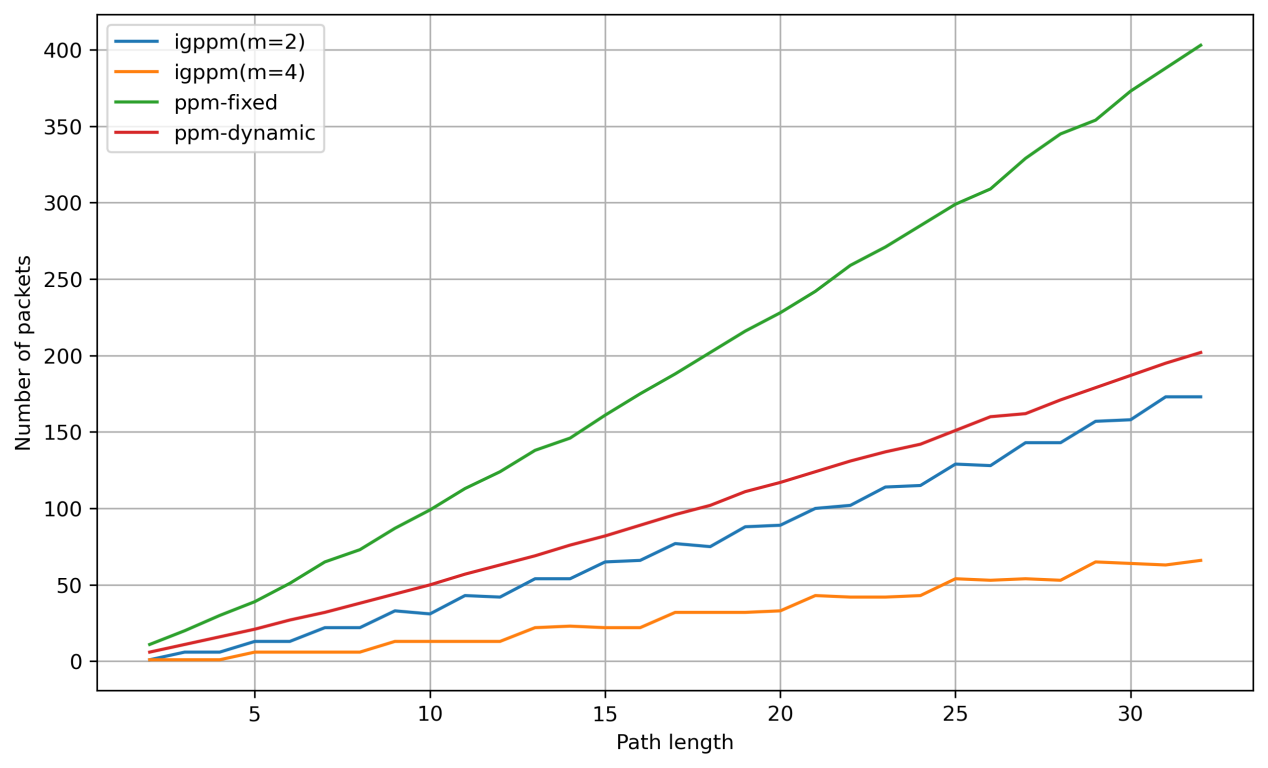
\includegraphics[width = 0.8\textwidth]{packets_num.png}
  \caption{路径重建所需数据包数量与路径长度关系(成功率 = 95\%)}
  \label{fig:packets_num}
\end{figure}   
可以看出,本文提出的方案在完成路径重构时所需要的数据包数量要远远少于PPM-Fixed方案。
当m=2时本方案略优于PPM-Dynamic方案,当m=4时则明显优于以上两种PPM类方案。另外,
仔细观察图像可以发现,本文提出的方案表现出阶梯性特征,这是因为该方案采用了分组
标记的方法:不管跳数d相差多少,只要$k = \lceil d/m \rceil$相同,完成路径重构所需
要的数据包数量就会相同。


在传统的PPM类方案中,完成路径重构所需的数据包数量通常指完成路由覆盖所需的数据包数量,
而非直接获得一条有序攻击路径的数据包数量。要想获得一条有序的攻击路径仍需要额外的操作,
例如网络探测、ISP网络地图等以确定具体的攻击路径。而在本方案中,可直接利用标记数据包
,获取接口号路径。之后再依据接口号路径,依次查询路由器便可获得一条有序的攻击路径。

\begin{figure}[htbp]
  \centering
  \subcaptionbox{数据包空间开销\label{fig:packet_overhead}}[0.44\textwidth]{
  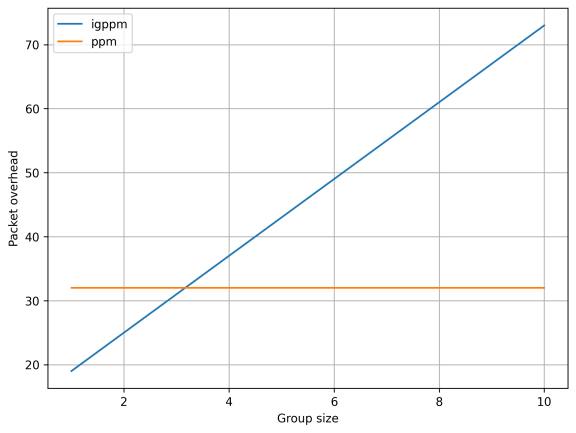
\includegraphics[width=0.45\textwidth]{packet_overhead.png}

  }
  \hspace{36pt}
  \subcaptionbox{数据包空间利用率\label{fig:space_utilization}}[0.44\textwidth]{
  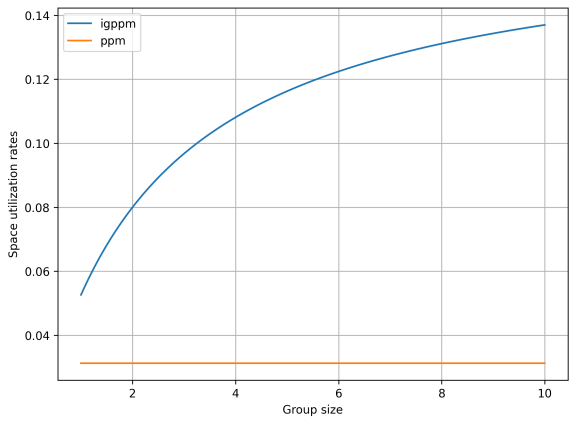
\includegraphics[width=0.46\textwidth]{space_utilization.png}
  }
  \caption{数据包空间开销即利用率与组大小关系}
\end{figure}
图~\ref*{fig:packet_overhead}~展示了本文所提方案与PPM方案在数据包标记空
间开销方面的对比结果。本文所提方案进行路由标记所需的空间与组大小m成正比。当m小
于4时,IGPPM产生的空间开销低于PPM。图~\ref*{fig:space_utilization}~则展示了标记空间利用率方面的对比结果。
利用率是指单个数据包中标记的路由数量与数据包标记空间开销的比率。可以观察到,与
PPM方案相比,我们的方案具有更高的空间利用率,这显著提高了方案的路由回溯能力。
\section{本章小结}
\label{sec:otherparts}
在网络通信中,由于缺乏IP地址验证机制,攻击者可以冒充其他用户,
导致各种网络攻击,例如DoS/DDoS攻击,并可能引发其他损害目标主
机声誉和利益的恶意活动。因此,IP地址跟踪解决方案变得至关重要。

尽管概率包标记法作为一种能够进行路由回溯的有效方法,并且具备自动回溯的能力
,但这种方法都有一定的缺点:使用IP地址作为标记信息来对单个路由器进行标记,
这将导致标记空间利用率低、路径重建过程需要收集的数据包数量大,并且不能直接提供有序的攻击路径。

因此,本文介绍了IGPPM方案,该方案利用路由器接口编号的局部
唯一性及其与IP地址相比相对较小的空间要求实现了IGPPM在单
个数据包上携带更多的路由器标记信息。此外,通过对异或特性
的有效使用,当收集到足够的数据包以实现路径覆盖时,IGPPM可以
直接提供有序的攻击路径。

最后,本文通过理论分析和实验比较表明,与传统的PPM的方案相比,我们的方法显著减少了在路由回溯过程中达到收敛状态所需的数据包数量,提高了回溯效率。
